\documentclass{tudelft-report}

%% Set up the bibliography
\usepackage{biblatex}
\addbibresource{report.bib}

%% Additional packages and commands
\usepackage{parskip}
\setlist{itemsep=-2pt} % Reducing white space in lists slightly
\renewcommand{\deg}{\si{\degree}\xspace} % Use \deg easily, everywhere
\usepackage{tcolorbox}

%% ----------------------------------------------------------------------
%%    Begin of document + Frontmatter (Roman page numbering)
%% ----------------------------------------------------------------------

\begin{document}

\frontmatter

%% Define the main parameters
\title{\textbf{Laboratorio} \\ Proyecto Final}
\author{Ingeniería Matemática}

\subject{Visión por Ordenador I} % Cover only
\affiliation{Universidad Pontificia Comillas, ICAI} % Cover only
\coverimage{figures/cover.png} % Aspect ratio of 2:3 (portrait) recommended
\definecolor{title}{HTML}{ffffff} % Color for cover title

\makecover

\begin{titlepage}

\begin{center}

\bigskip
\bigskip

%% Print the name of the author
{\makeatletter
\begin{tabular}{c}
    3º \@author \\\midrule
    Curso 2024/25
\end{tabular}
\makeatother}

\bigskip
\bigskip

%% Print the title
{\makeatletter
\largetitlestyle\fontsize{45}{45}\selectfont\@title
\makeatother}

%% Print the subtitle
{\makeatletter
\ifdefvoid{\@subtitle}{}{\bigskip\titlestyle\fontsize{20}{20}\selectfont\@subtitle}
\makeatother}

%% Print table with names; easily add columns if necessary or remove the table completely
% \setlength\extrarowheight{2pt}
% \begin{tabular}{c}
%     3º  \\\midrule
%     Curso 2024/25 \\
% \end{tabular}

\vfill

%% Print some more information at the bottom
\begin{tabular}{ll}
    \textbf{Profesor}: & \textbf{Email} \\
    Erik Velasco & evelasco@icai.comillas.edu \\
    Lionel Güitta & lglopez@icai.comillas.edu \\
    Daniel Pinilla & dpinilla@icai.comillas.edu \\
    Luis Arias & learias@icai.comillas.edu \\
    Rodrigo Sánchez & rsmolina@icai.comillas.edu \\ 
    Ignacio de Rodrigo & iderodrigo@comillas.edu \\
\end{tabular}

\bigskip
\bigskip

%% Add a source and description for the cover and optional attribution for the template
\begin{tabular}{p{15mm}p{10cm}}
    Cover: & Canadarm 2 Robotic Arm Grapples SpaceX Dragon by NASA under CC BY-NC 2.0 (Modified) \\
    % Feel free to remove the following attribution, it is not required - still appreciated :-)
    % Style: & TU Delft Report Style, with modifications by Daan Zwaneveld
\end{tabular}
\vspace{10mm}

\end{center}

%% Insert the TU Delft logo at the bottom of the page
\begin{tikzpicture}[remember picture, overlay]
    \node[above=10mm] at (current page.south) {%
        
\includegraphics[scale=0.15]{figures/logo-color}
    };
\end{tikzpicture}

\end{titlepage}

%\chapter*{Preface}
\addcontentsline{toc}{chapter}{Preface}

\emph{A preface...}

\begin{flushright}
{\makeatletter\itshape
    \@author \\
    Delft, \monthname{} \the\year{}
\makeatother}
\end{flushright}

%\chapter*{Summary}
\addcontentsline{toc}{chapter}{Summary}

\emph{A summary...}


\tableofcontents
%\listoffigures
%\listoftables

%\chapter*{Nomenclature}
\addcontentsline{toc}{chapter}{Nomenclature}

\emph{If a nomenclature is required, a simple template can be found below for convenience. Feel free to use, adapt or completely remove.}

\section*{Abbreviations}

\begin{longtable}{p{2.5cm}p{8cm}}
    \toprule
    Abbreviation & Definition \\
    \midrule\endhead % Add abbreviations alphabetically here:
    ISA & International Standard Atmosphere \\
    ... \\
    \bottomrule
\end{longtable}

\section*{Symbols}

\begin{longtable}{p{2.5cm}p{8cm}p{2.5cm}}
    \toprule
    Symbol & Definition & Unit \\
    \midrule\endhead % Add Latin symbols alphabetically here:
    $V$ & Velocity & [m/s] \\
    ... \\
    \midrule % Add Greek symbols alphabetically here:
    $\rho$ & Density & [kg/m$^3$] \\
    ... \\
    \bottomrule
\end{longtable}


%% ----------------------------------------------------------------------
%%    Mainmatter (Arabic page numbering)
%% ----------------------------------------------------------------------

\mainmatter

\chapter{Proyecto Final: \textbf{Introducción}}
\label{chapter:introduction_lab_project}

Una vez realizadas las cuatro sesiones prácticas (calibración, procesamiento de imágenes, extracción de características y detección de objetos), se tienen los conocimientos necesarios para implementar proyectos sencillos de Visión por Ordenador. Aunque basados en conceptos básicos, la combinación de los módulos vistos en las sesiones prácticas puede alcanzar resultados muy potentes. 

En este proyecto se debe idear e implementar un sistema de visión (clásica) por ordenador utilizando una Raspberry Pi y una cámara como entrada de información al sistema. El campo de aplicación es libre (medicina, deportes, seguridad...) y se os anima a ser originales. 

El objetivo de este proyecto no es solo evaluar sus capacidades técnicas, sino que también se persigue que el resultado final sirva como parte de su porfolio. De este modo, se anima a que el resultado final del proyecto sea un vídeo (demo) y un documento pulido.

\chapter{\textbf{Materiales}}
\label{chapter:materiales}

\subsection*{Hardware}
\phantomsection
\addcontentsline{toc}{section}{Hardware}
\vspace{5mm}

Tal y como se menciona en la Introducción, el proyecto cuenta con un hardware específico (Figura \ref{fig:materials}, Raspberry Pi y cámara) que se entregará durante la primera sesión dedicada al trabajo. Su uso es obligatorio. 

En casos especiales donde el proyecto requiera algún elemento de hardware más complejo (impresión 3D, electrónica, etc.) se recomienda comunicarlo a los profesores lo antes posible (especialmente en el caso de impresión 3D, pues hay que consultar disponibilidad en la Universidad).

Por otro lado, desde el punto de vista de software, se puede hacer uso de cualquier librería, aunque el uso de modelos avanzados de Visión por Ordenador (Deep Learning) debe consultarse con los profesores ya que no es el objetivo de esta asignatura. Por último, también está disponible el uso de una Api Key de OpenAI para proyectos en los que pueda aportar valor.

\begin{figure}[H]
    \centering
    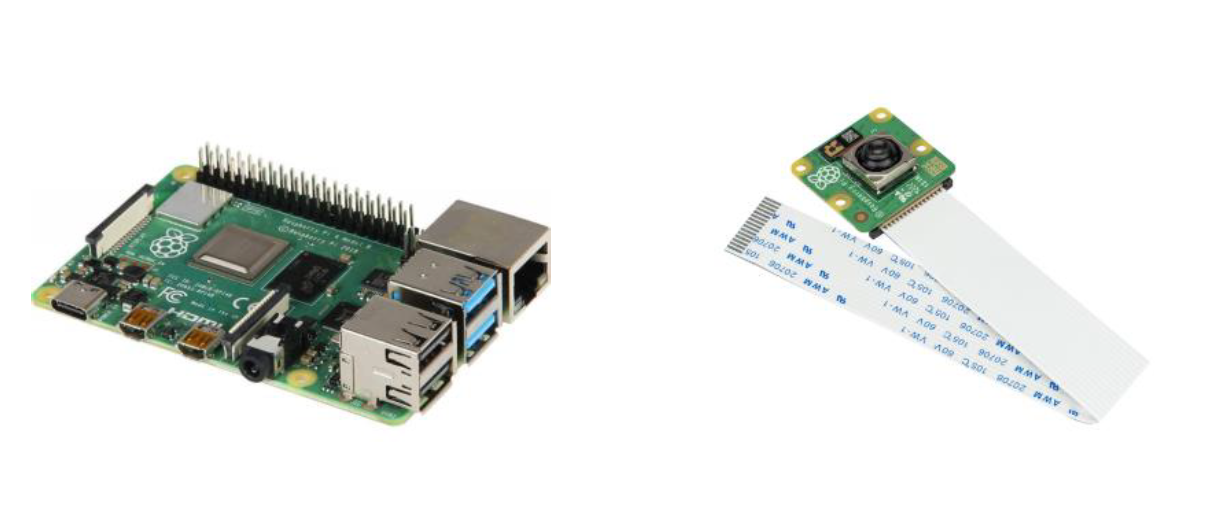
\includegraphics[width=0.65\textwidth]{Lab_Project/template/figures/materials.png}
    \caption{Materiales básicos pro porcionados: Raspberry Pi 4 y Cámara.}
    \label{fig:materials}
\end{figure}

\chapter{\textbf{Requisitos y Tareas}}
\label{chapter:requisitos}

\subsection*{Hardware}
\phantomsection
\addcontentsline{toc}{section}{Hardware}
\vspace{5mm}

\begin{itemize}
    \item \textbf{Raspberry Pi}: es imprescindible el uso de la Raspberry Pi. En ella se alojará el sistema diseñado.
    \item \textbf{Cámara}: es imprescindible el uso de la cámara como entrada de datos del sistema.
\end{itemize}

\subsection*{Software}
\phantomsection
\addcontentsline{toc}{section}{Software}
\vspace{5mm}

\begin{itemize}
    \item \textbf{Calibración}: es imprescindible implementar la calibración de la cámara utilizando un patrón que diseñéis vosotros, así como un método de calibración de implementación propia. En el informe se deberán incluir los valores resultantes de la calibración, incluido el RMS.
    \item \textbf{Detección de patrones}: Se deberá implementar un módulo capaz de diferenciar patrones sencillos a través de procesado de imagen: líneas negras sobre fondo blanco, círculos, etc. Se valorará el método de detección de estos patrones, así como el diseño de los mismos.
    \item \textbf{Extracción de información}: se debe implementar un decodificador que memorice hasta 4 patrones consecutivos y garantice o bloquee el paso al siguiente bloque en función de si estos patrones están en el orden correcto o no. El alumno deberá implementar para ello una lógica que permita memorizar esta secuencia y resetear u olvidarla cuando se necesite.
    \item \textbf{Tracker}: al introducir la secuencia de patrones correcta, se ejecutará el tracker que deberá mostrar por pantalla una bounding box alrededor de la zona de interés que aparezca en la imagen y seguirla mientras se mueve. La explicación del algoritmo de la detección y su monitorización deberá incluirse en el informe final del proyecto.
    \item \textbf{Módulos mínimos}: Salida de vídeo, calibración, detección de al menos un tipo de patrón, decodificador de secuencia y tracker.
    \item \textbf{Cualquier propuesta adicional al planteamiento inicial del proyecto se valorará positivamente}: nuevos módulos, distintos modos de funcionamiento, etc.
    \item \textbf{Real time}: se valorará positivamente también que el código esté optimizado. Es fundamental que tengáis esto en mente. De nada sirve un algoritmo de detección de patrones si luego no funciona a una tasa de refresco lo suficientemente rápida como para que sea útil. Esto también permite que este proyecto se pueda integrar con otros, como puede ser en la asignatura de robots del segundo cuatrimestre.
\end{itemize}
\chapter{\textbf{Metodología}}
\label{chapter:metodologia}

\subsection*{Diagramas de bloques}
\phantomsection
\addcontentsline{toc}{section}{Diagramas de bloques}
\vspace{5mm}

\begin{itemize}
    \item \textbf{Diagrama de bloques del sistema}: es imprescindible presentar en el informe un diagrama de bloques que explique la arquitectura del sistema implementado.
    \item \textbf{Diagrama de bloques de la imagen}: en casos donde el diagrama de bloques del sistema deba abstraerse demasiado para la comprensión del proyecto, será necesario realizar un diagrama de bloques particular para la imagen donde se muestre cómo se procesa.
\end{itemize}

La Figura \ref{fig:diagrama} muestra un resumen de los módulos de software y pueden ayudarle a esbozar sistema (y diagramas).

\begin{figure}[H]
    \centering
    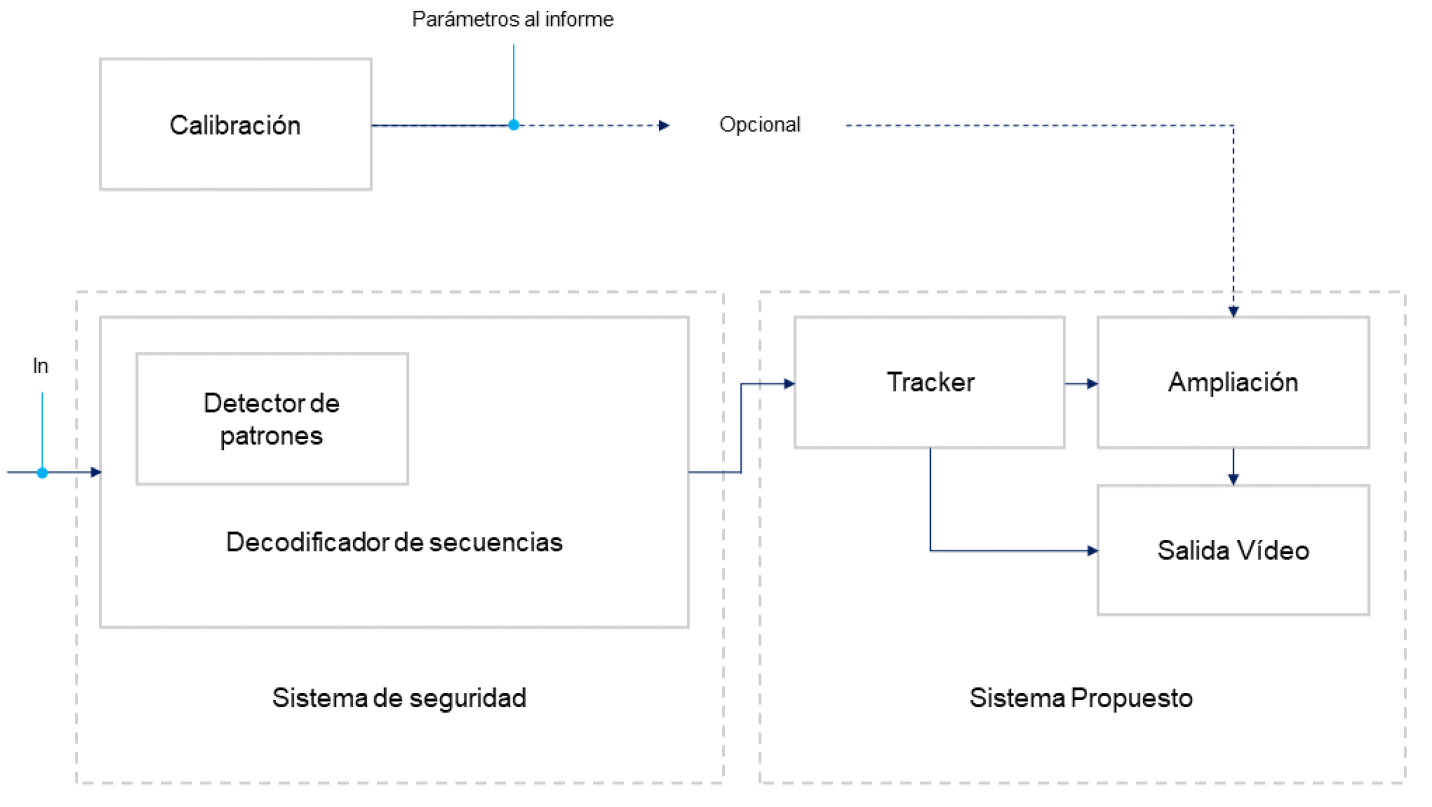
\includegraphics[width=0.85\textwidth]{Lab_Project/template/figures/diagrama.png}
    \caption{Sistema con módulos mínimos. En el módulo calibración se deberá implementar el método de calibración y el de corrección de la distorsión.}
    \label{fig:diagrama}
\end{figure}
\chapter{\textbf{Fechas y Entregables}}
\label{chapter:fechas_entregables}

\subsection*{Fechas}
\phantomsection
\addcontentsline{toc}{section}{Fechas}
\vspace{5mm}

\begin{itemize}
    \item \textbf{Inicio del proyecto}: 15-19 de noviembre de 2024.
    \item \textbf{Aprobación de los contenidos del proyecto}: 22-26 de noviembre de 2024.
    \item \textbf{Entrega final del proyecto}: 10 de enero de 2025
\end{itemize}

\subsection*{Entregables}
\phantomsection
\addcontentsline{toc}{section}{Entregables}
\vspace{5mm}

\begin{itemize}
    \item \textbf{Código en GitHub}: público con ReadMe completo y bien estructurado.
    \item \textbf{Vídeo}: en el que se hará una demo del proyecto y se explicará con el apoyo de un póster o PPT tipo brochure. El vídeo debe incrustar en sus frames la tasa de refresco a la que se ejecuta el sistema (FPS).
    \item \textbf{Informe}: de máximo 5 páginas, donde se incluyan los siguientes puntos:
    \begin{itemize}
        \item \textbf{Introducción}: alcance del proyecto.
        \item \textbf{Metodología}: cómo se ejecuta:
        \begin{itemize}
            \item Calibración de la cámara.
            \item Diagrama de bloques del sistema.
            \item Secuencia de transformación de la imagen.
            \item Sistema de seguridad: Detección de patrones y Extracción de información.
            \item Sistema propuesto: tracker, ampliaciones y salida de vídeo.
        \end{itemize}
        \item \textbf{Resultados}
        \item \textbf{Futuros Desarrollos}
    \end{itemize}
\end{itemize}
\chapter{\textbf{Calificaciones}}
\label{chapter:calificaciones}

\subsection*{Criterios}
\phantomsection
\addcontentsline{toc}{section}{Criterios}
\vspace{5mm}


El proyecto final se calificará de acuerdo a los apartados de la Tablas \ref{table:evaluacionI} y \ref{table:evaluacionII}. La nota final del proyecto se calculará según la Fórmula \ref{eq:final_grade}.

\begin{align}
     \text{Calficación} &= N \times F
    \label{eq:final_grade}
\end{align}

\begin{table}[h!]
    \centering
    \begin{tabular}{|l|c|c|}
    \hline
    \textbf{Módulos} & \textbf{Valor} & \textbf{Resultado} \\
    \hline
    Calibración & 1.0 & \\
    \hline
    Detector de patrones & 2.0 & \\
    \hline
    Extracción de información & 2.0 & \\
    \hline
    Tracker & 2.0 & \\
    \hline
    Salida de vídeo & 1.0 & \\
    \hline
    Tiempo real & 1.0 (extra) & \\
    \hline
    Ampliaciones & 2.0 & \\
    \hline
    \hline
    \textbf{Nota} & \textbf{11.0} & N \\
    \hline
    \end{tabular}
    \caption{Valoración de los apartados del proyecto final.}
    \label{table:evaluacionI}
\end{table}

\begin{table}[h!]
    \centering
    \begin{tabular}{|l|c|c|}
    \hline
    \textbf{Factores} & \textbf{Peso} & \textbf{Resultado} \\
    \hline
    Informe & 0.50 & \\
    \hline
    Repositorio & 0.25 & \\
    \hline
    Vídeo & 0.25 & \\
    \hline
    \hline
    \textbf{Factor} & \textbf{1.0} & F\\
    \hline
    \end{tabular}
    \caption{Factores .}
    \label{table:evaluacionII}
\end{table}
\chapter{\textbf{Primeros Pasos}}
\label{chapter:primeros_pasos}

\subsection*{Hardware}
\phantomsection
\addcontentsline{toc}{section}{Hardware}
\vspace{5mm}

Al comienzo de la sesión dispondrá de:

\begin{itemize}
    \item \textbf{Raspberry Pi}.
    \item \textbf{Camera module 3 WIDE (120º FOV)}.
    \item \textbf{Cable de alimentación a USB3}.
    \item \textbf{Cable HDMI to micro-HDMI (opcional)}
\end{itemize}

Realice el montaje según las indicaciones de su profesor. Todas las Rasspberry tienen flasheadas un sistema operativo compatible y con SSH activado. Aunque se recomienda el uso de un cable HDMI para facilitar el proceso, puede acceder a su Raspberry de múltiples formas:

Puede encontrar la IP address de su placa o su \textit{host name} para conectarse, o bien por SSH (SSH host-name.local) o por VNC (connect to host-name). Para conectarse por SSH puede utilizar Putty. Para conectarte por VNC puede usar RealVNC. No es necesario usar un programa concreto para la conexión con la Raspberry, use el que mejor se adecúe a sus necesidades. Regístrese con las credenciales de la Tabla \ref{table:credenciales}:

\begin{table}[h!]
    \centering
    \begin{tabular}{|l|l|}
    \hline
    \textbf{Campo} & \textbf{Valor}\\
    \hline
    Usuario & pi \\
    \hline
    Contraseña & imat@ICAI2024 \\
    \hline
    IP (Comillas) & 10.120.107.<número> \\
    \hline
    Nombre del equipo (hostname) en Comillas & imat-rpi-<xyz>.rpi-deac.alumnos.upcont.es \\
    \hline
    Nombre del equipo en otra red & imat-rpi-<xyz> \\
    \hline
    \end{tabular}
    \caption{Credenciales para iniciar sesión en la Raspberry Pi. Tenga en cuenta que <número> es el código de la placa que le han dado (por ejemplo 42), mientras que código <xyz> es el mismo número precedido por 0 (por ejemplo 042).}
    \label{table:credenciales}
\end{table}

Para comprobar que la cámara está conectada, ejecute el archivo que encontrará en la carpeta del projecto final: \texttt{test.py}. Como resultado, si se ha conectado directamente a un monitor, o si lo ha hecho con escritorio remoto, debería ver el vídeo captado por la cámara en tiempo real.

Si trabaja de manera cómoda implementando el código directamente en la Raspberry, puede optar por instalar Visual Studio Code desde el terminal de su Raspberry. Esta es una buena opción, puesto que podrá integrar el soporte Git de VSCode directamente. Utilice los siguientes comandos:\\

\texttt{sudo apt-get update}\\
\texttt{sudo apt-get install code}

\subsection*{Sesión Inicial}
\phantomsection
\addcontentsline{toc}{section}{Sesión Inicial}
\vspace{5mm}
En la primera sesión se espera que se aborden los siguientes puntos:

\begin{itemize}
    \item \textbf{Montaje}: Conexión con la Raspberry. Acceso con escritorio remoto, SSH o mediante cable HDMI.
    \item \textbf{Conexión} de cámara y recepción de vídeo.
    \item \textbf{Repositorio del proyecto}. Primer commit con el código de lectura de vídeo desde la cámara. Recuerde que se debe crear un ReadMe con la descripción del proyecto. Deberá hacer el proyecto público y compartir el enlace al mismo con el profesor.
    \item  \textbf{Planteamiento y diseño del proyecto}. Recuerde que antes de implementar su proyecto, debe contar con la aprobación del profesor.
\end{itemize}

%% Prevent urls running into margins in bibliography
\setcounter{biburlnumpenalty}{7000}
\setcounter{biburllcpenalty}{7000}
\setcounter{biburlucpenalty}{7000}

%% Add bibliography
% \printbibliography[heading=bibintoc,title=References]

%% ----------------------------------------------------------------------
%%    Appendix (Letters for chapters)
%% ----------------------------------------------------------------------

%\appendix

%\chapter{Source Code Example}
%\label{chapter:title}

\emph{Adding source code to your report/thesis is supported with the package {\normalfont\texttt{listings}}. An example can be found below. Files can be added using {\normalfont\texttt{\textbackslash lstinputlisting[language=<language>]\{<filename>\}}}.}

\begin{lstlisting}[language=Python]
"""
ISA Calculator: import the function, specify the height and it will return a
list in the following format: [Temperature,Density,Pressure,Speed of Sound].
Note that there is no check to see if the maximum altitude is reached.
"""

import math
g0 = 9.80665
R = 287.0
layer1 = [0, 288.15, 101325.0]
alt = [0,11000,20000,32000,47000,51000,71000,86000]
a = [-.0065,0,.0010,.0028,0,-.0028,-.0020]

def atmosphere(h):
    for i in range(0,len(alt)-1):
        if h >= alt[i]:
            layer0 = layer1[:]
            layer1[0] = min(h,alt[i+1])
            if a[i] != 0:
                layer1[1] = layer0[1] + a[i]*(layer1[0]-layer0[0])
                layer1[2] = layer0[2] * (layer1[1]/layer0[1])**(-g0/(a[i]*R))
            else:
                layer1[2] = layer0[2]*math.exp((-g0/(R*layer1[1]))*(layer1[0]-layer0[0]))
    return [layer1[1],layer1[2]/(R*layer1[1]),layer1[2],math.sqrt(1.4*R*layer1[1])]
\end{lstlisting}

%\chapter{Task Division Example}
%\label{chapter:title}

\emph{If a task division is required, a simple template can be found below for convenience. Feel free to use, adapt or completely remove.}

\begin{table}[htb]
    \setlength\extrarowheight{4pt}
    \centering
    \caption{Distribution of the workload}
    \label{tab:taskdivision}
    \begin{tabularx}{\textwidth}{lXX}
        \toprule
        & Task & Student Name(s) \\
        \midrule
        & Summary & \\
        Chapter 1 & Introduction &  \\
        Chapter 2 &  & \\
        Chapter 3 &  & \\
        Chapter * &  & \\
        Chapter * & Conclusion &  \\
        \midrule
        & Editors & \\
        & CAD and Figures & \\
        & Document Design and Layout & \\
        \bottomrule
    \end{tabularx}
\end{table}

%\input{appendix/appendix-c} % Create file to add

\end{document}
